\documentclass[12pt, a4paper]{report}

% ===== PACKAGES =====
\usepackage[utf8]{inputenc}
\usepackage[T5]{fontenc}
\usepackage[vietnamese,english]{babel}
\usepackage{geometry}
\usepackage{graphicx}
\usepackage{amsmath, amssymb, amsfonts}
\usepackage{booktabs}
\usepackage{longtable}
\usepackage{array}
\usepackage{multirow}
\usepackage{xcolor}
\usepackage{hyperref}
\usepackage{listings}
\usepackage{enumitem}
\usepackage{fancyhdr}
\usepackage{titlesec}
\usepackage{caption}
\usepackage{subcaption}
\usepackage{float}
\usepackage{setspace}
\usepackage{indentfirst}
\usepackage{tocbibind}
\usepackage{algorithm}
\usepackage{algpseudocode}
\graphicspath{{../../}{./}}

% ===== PAGE LAYOUT =====
\geometry{
  top=2.5cm,
  bottom=2.5cm,
  left=3cm,
  right=2cm
}
\onehalfspacing

% ===== COLORS =====
\definecolor{codegreen}{rgb}{0,0.6,0}
\definecolor{codegray}{rgb}{0.5,0.5,0.5}
\definecolor{codepurple}{rgb}{0.58,0,0.82}
\definecolor{backcolour}{rgb}{0.97,0.97,0.97}
\definecolor{primaryblue}{RGB}{0,84,166}

% ===== CODE STYLE =====
\lstdefinestyle{mystyle}{
  backgroundcolor=\color{backcolour},
  commentstyle=\color{codegreen},
  keywordstyle=\color{primaryblue}\bfseries,
  numberstyle=\tiny\color{codegray},
  stringstyle=\color{codepurple},
  basicstyle=\ttfamily\small,
  breakatwhitespace=false,
  breaklines=true,
  captionpos=b,
  keepspaces=true,
  numbers=left,
  numbersep=5pt,
  showspaces=false,
  showstringspaces=false,
  showtabs=false,
  tabsize=2,
  frame=single,
  rulecolor=\color{gray!40}
}
\lstset{style=mystyle}

% ===== HYPERREF =====
\hypersetup{
  colorlinks=true,
  linkcolor=primaryblue,
  urlcolor=primaryblue,
  citecolor=primaryblue,
  pdftitle={Báo cáo: Bài toán Tập Thống Trị Tối Thiểu},
  pdfauthor={Nhóm 5 - Thiết kế và Đánh giá thuật toán}
}

% ===== HEADER & FOOTER =====
\pagestyle{fancy}
\fancyhf{}
\fancyhead[L]{\small\textit{Bài toán Tập Thống Trị Tối Thiểu}}
\fancyhead[R]{\small\textit{Nhóm 5}}
\fancyfoot[C]{\thepage}
\renewcommand{\headrulewidth}{0.4pt}

% ===== CHAPTER STYLE =====
\titleformat{\chapter}[block]
  {\normalfont\LARGE\bfseries\color{primaryblue}}
  {\chaptername\ \thechapter:}{1em}{}
\titlespacing*{\chapter}{0pt}{20pt}{15pt}

% ===== CUSTOM COMMANDS =====
\newcommand{\MDS}{\textsc{Minimum Dominating Set}}
\newcommand{\OPT}{\mathrm{OPT}}
\newcommand{\closedN}[1]{N[#1]}

\begin{document}
\selectlanguage{vietnamese}

% ===== COVER PAGE =====
\begin{titlepage}
  \centering
  \textbf{\large TRƯỜNG ĐẠI HỌC KHOA HỌC TỰ NHIÊN -- ĐHQGHN}\\[0.3cm]
  \textbf{\large Khoa Toán -- Cơ -- Tin học}\\[0.5cm]
  \rule{\linewidth}{0.5pt}\\[1cm]

  {\large\textit{Môn học: Thiết kế và Đánh giá thuật toán}}\\[2cm]

  {\Huge\bfseries\color{primaryblue} BÀI TOÁN TẬP THỐNG TRỊ\\[0.3cm] TỐI THIỂU}\\[0.5cm]
  {\Large\textbf{MINIMUM DOMINATING SET ALGORITHMS}}\\[2cm]

  \textbf{Đề tài:} Thiết kế, cài đặt và đánh giá các thuật toán giải bài toán tập thống trị tối thiểu\\[1cm]

  \begin{tabular}{|c|l|l|}
    \hline
    \textbf{Mã sinh viên} & \textbf{Họ và tên} & \textbf{Vai trò} \\
    \hline
    23001917 & Hoàng Minh Quang & Trưởng nhóm \\
    23001918 & Nguyễn Đức Quang & Thành viên \\
    23001929 & Nguyễn Thành Tâm & Thành viên \\
    23001926 & Nguyễn Thế Tài & Thành viên \\
    \hline
  \end{tabular}\\[2cm]

  \textit{Hà Nội, tháng 5 năm 2026}
\end{titlepage}

\tableofcontents
\listoffigures
\listoftables
\newpage

% =============================================================
\chapter{Giới thiệu}

\section{Đặt vấn đề}

Trong nhiều bài toán tối ưu trên mạng lưới, ta cần chọn một số lượng nhỏ các điểm trung tâm sao cho
mọi điểm còn lại đều được phục vụ trực tiếp hoặc thông qua liên kết gần nhất. Ví dụ, trong bài toán đặt
trạm phát sóng, đặt đồn cảnh sát, chọn máy chủ giám sát mạng hoặc chọn người đại diện trong mạng xã
hội, mục tiêu chung là giảm chi phí triển khai nhưng vẫn đảm bảo độ phủ toàn bộ hệ thống.

Bài toán \MDS{} mô hình hóa trực tiếp nhu cầu trên. Cho đồ thị vô hướng $G=(V,E)$, cần tìm tập
$D \subseteq V$ có số phần tử nhỏ nhất sao cho mọi đỉnh trong đồ thị hoặc thuộc $D$, hoặc kề với ít nhất
một đỉnh thuộc $D$. Tập $D$ như vậy được gọi là tập thống trị; tập thống trị có kích thước nhỏ nhất được
gọi là tập thống trị tối thiểu.

\section{Mục tiêu đề tài}

Đề tài hướng đến bốn mục tiêu chính:

\begin{enumerate}[leftmargin=*, label=\arabic*.]
  \item Phân tích hình thức bài toán \MDS{}, bao gồm mô hình hóa, điều kiện hợp lệ và độ khó tính toán.
  \item Thiết kế và cài đặt nhiều hướng giải: vét cạn, nhánh cận, tham lam và tối ưu đàn kiến.
  \item Chứng minh tính đúng đắn cho các thuật toán chính xác, đồng thời phân tích độ phức tạp của
    toàn bộ các thuật toán được cài đặt.
  \item Thực nghiệm trên các đồ thị ngẫu nhiên có quy mô và mật độ khác nhau để so sánh thời gian chạy,
    chất lượng nghiệm, ưu điểm và nhược điểm của từng thuật toán.
\end{enumerate}

\section{Phạm vi thực hiện}

Project tập trung vào đồ thị vô hướng, không trọng số. Dữ liệu đầu vào được biểu diễn bằng danh sách kề
\texttt{adj}, trong đó \texttt{adj[v]} là tập các đỉnh kề với đỉnh $v$. Các thuật toán được cài đặt bằng
Python, kết quả benchmark được lưu tại thư mục \texttt{results/}, gồm dữ liệu thô, bảng tổng hợp và biểu đồ.

\section{Cấu trúc báo cáo}

Báo cáo gồm 7 chương. Chương 2 trình bày cơ sở lý thuyết và phân tích bài toán. Chương 3 mô tả thiết
kế thuật toán. Chương 4 chứng minh tính đúng đắn và phân tích độ phức tạp. Chương 5 trình bày cài đặt
và dữ liệu thực nghiệm. Chương 6 đánh giá kết quả. Chương 7 kết luận và định hướng phát triển.

% =============================================================
\chapter{Cơ sở lý thuyết và phân tích bài toán}

\section{Các khái niệm đồ thị}

Cho đồ thị vô hướng $G=(V,E)$, với $V=\{0,1,\ldots,n-1\}$ là tập đỉnh và $E \subseteq V \times V$ là
tập cạnh. Hai đỉnh $u,v$ được gọi là kề nhau nếu $(u,v)\in E$. Tập láng giềng mở của $v$ là:

\begin{equation}
  N(v)=\{u \in V \mid (u,v)\in E\}.
\end{equation}

Tập láng giềng đóng của $v$ là:

\begin{equation}
  N[v]=N(v)\cup\{v\}.
\end{equation}

Với một tập đỉnh $D \subseteq V$, tập các đỉnh được $D$ phủ là:

\begin{equation}
  \mathrm{cover}(D)=\bigcup_{v\in D} N[v].
  \label{eq:cover}
\end{equation}

\section{Định nghĩa bài toán}

\textbf{Tập thống trị.} Một tập $D \subseteq V$ được gọi là tập thống trị của $G$ nếu:

\begin{equation}
  \forall u \in V,\quad u \in D \ \text{hoặc}\ \exists v \in D: (u,v)\in E.
\end{equation}

Tương đương:

\begin{equation}
  \mathrm{cover}(D)=V.
\end{equation}

\textbf{Tập thống trị tối thiểu.} Bài toán \MDS{} yêu cầu tìm tập thống trị $D^*$ sao cho:

\begin{equation}
  |D^*|=\min\{|D| \mid D \subseteq V,\ \mathrm{cover}(D)=V\}.
  \label{eq:mds}
\end{equation}

Giá trị $|D^*|$ thường được gọi là số thống trị của đồ thị, ký hiệu $\gamma(G)$.

\section{Ví dụ minh họa}

Xét đồ thị đường đi $P_5$ gồm 5 đỉnh:

\[
  0 - 1 - 2 - 3 - 4.
\]

Tập $D=\{1,3\}$ là tập thống trị vì:

\[
  N[1]\cup N[3]=\{0,1,2\}\cup\{2,3,4\}=V.
\]

Không tồn tại tập thống trị có một đỉnh, do không có đỉnh nào kề hoặc bằng toàn bộ 5 đỉnh. Vì vậy
$D=\{1,3\}$ là một tập thống trị tối thiểu và $\gamma(P_5)=2$.

\section{Mô hình hóa như bài toán Set Cover}

Bài toán \MDS{} có thể được chuyển về bài toán phủ tập. Với mỗi đỉnh $v\in V$, tạo một tập:

\begin{equation}
  S_v=N[v].
\end{equation}

Khi chọn đỉnh $v$ vào tập thống trị, ta tương đương với chọn tập $S_v$ để phủ các đỉnh trong $N[v]$.
Do đó, \MDS{} trở thành bài toán chọn ít tập nhất trong $\{S_v \mid v\in V\}$ sao cho hợp của chúng
bằng $V$. Cách nhìn này giải thích vì sao thuật toán tham lam chọn đỉnh phủ được nhiều đỉnh chưa phủ
nhất là một lựa chọn tự nhiên.

\section{Độ khó của bài toán}

Phiên bản quyết định của bài toán là:

\begin{quote}
  Cho đồ thị $G=(V,E)$ và số nguyên $k$, có tồn tại tập thống trị $D$ sao cho $|D|\leq k$ hay không?
\end{quote}

Bài toán quyết định này thuộc lớp NP vì với một tập $D$ cho trước, ta có thể kiểm tra $D$ có phải tập
thống trị và $|D|\leq k$ trong thời gian đa thức. Bài toán cũng là NP-complete; do đó phiên bản tối ưu
\MDS{} là NP-hard. Hệ quả thực tế là khó kỳ vọng có thuật toán đa thức luôn tìm nghiệm tối ưu cho mọi
đồ thị tổng quát, trừ khi $P=NP$.

Vì vậy, project triển khai hai nhóm thuật toán:

\begin{itemize}
  \item \textbf{Thuật toán chính xác}: vét cạn và nhánh cận, đảm bảo tìm nghiệm tối ưu nhưng khó mở rộng
    cho $n$ lớn.
  \item \textbf{Thuật toán xấp xỉ/heuristic}: tham lam và ACO, chạy được trên đồ thị lớn hơn nhưng không
    đảm bảo tối ưu tuyệt đối.
\end{itemize}

% =============================================================
\chapter{Thiết kế và xây dựng thuật toán}

\section{Biểu diễn dữ liệu}

Project biểu diễn đồ thị bằng danh sách kề:

\begin{lstlisting}[language=Python, caption={Biểu diễn đồ thị bằng danh sách kề}]
adj = [
    {1, 2},     # neighbors of vertex 0
    {0, 3},     # neighbors of vertex 1
    {0, 4},     # neighbors of vertex 2
    {1, 5},     # neighbors of vertex 3
    {2, 6},     # neighbors of vertex 4
    {3, 6},     # neighbors of vertex 5
    {4, 5},     # neighbors of vertex 6
]
\end{lstlisting}

Hàm kiểm tra một tập $D$ có thống trị toàn bộ đồ thị hay không được xây dựng theo công thức
\ref{eq:cover}: khởi tạo \texttt{covered = set(D)}, sau đó hợp thêm các tập kề của từng đỉnh trong $D$.
Nếu \texttt{len(covered) == n}, tập $D$ hợp lệ.

\section{Thuật toán vét cạn}

\subsection{Ý tưởng}

Thuật toán vét cạn thử toàn bộ tập con của $V$ theo thứ tự kích thước tăng dần. Với mỗi kích thước
$k=1,2,\ldots,n$, thuật toán sinh tất cả tổ hợp $k$ đỉnh và kiểm tra tổ hợp đó có phải tập thống trị
không. Tập hợp lệ đầu tiên tìm được chính là nghiệm tối ưu.

\begin{algorithm}[H]
\caption{Vét cạn cho bài toán \MDS{}}
\begin{algorithmic}[1]
\Require Đồ thị $G=(V,E)$
\Ensure Tập thống trị tối thiểu $D$
\For{$k \gets 1$ to $|V|$}
  \ForAll{$D \subseteq V$ sao cho $|D|=k$}
    \If{$\mathrm{cover}(D)=V$}
      \State \Return $D$
    \EndIf
  \EndFor
\EndFor
\State \Return $V$
\end{algorithmic}
\end{algorithm}

\subsection{Đặc điểm}

Vét cạn đơn giản, dễ kiểm chứng và phù hợp làm chuẩn tối ưu cho thực nghiệm nhỏ. Nhược điểm lớn nhất
là số tập con tăng theo $2^n$, khiến thuật toán không khả thi khi $n$ lớn.

\section{Thuật toán nhánh cận}

\subsection{Ý tưởng}

Nhánh cận vẫn tìm nghiệm tối ưu nhưng giảm số trạng thái phải duyệt bằng cắt nhánh. Tại một trạng thái,
giả sử ta đã chọn tập hiện tại $D$ và đã phủ được tập \texttt{dominated}. Nếu chưa phủ hết đồ thị, thuật
toán chọn một đỉnh chưa được phủ $u$. Để $u$ được thống trị, nghiệm cuối cùng bắt buộc phải chọn $u$
hoặc một đỉnh kề với $u$. Vì vậy, thuật toán chỉ cần phân nhánh trên tập ứng viên:

\begin{equation}
  C(u)=N[u].
\end{equation}

Project dùng nghiệm tham lam làm cận trên ban đầu. Ngoài ra, tại mỗi trạng thái, nếu ngay cả trong trường
hợp tốt nhất cũng không thể cải thiện nghiệm tốt nhất hiện có, nhánh đó bị loại bỏ.

\subsection{Cận dưới}

Gọi $\Delta$ là bậc lớn nhất của đồ thị. Một đỉnh có thể phủ tối đa $\Delta+1$ đỉnh, bao gồm chính nó
và các láng giềng. Nếu hiện còn $r$ đỉnh chưa được phủ, số đỉnh tối thiểu cần chọn thêm không thể nhỏ hơn:

\begin{equation}
  LB=\left\lceil \frac{r}{\Delta+1} \right\rceil.
  \label{eq:lower-bound}
\end{equation}

Nếu $|D|+LB \geq |D_{\mathrm{best}}|$, nhánh hiện tại không thể tạo nghiệm tốt hơn nghiệm tốt nhất đã biết,
do đó có thể cắt.

\begin{algorithm}[H]
\caption{Nhánh cận cho bài toán \MDS{}}
\begin{algorithmic}[1]
\Require Đồ thị $G=(V,E)$
\Ensure Tập thống trị tối thiểu $D_{\mathrm{best}}$
\State $D_{\mathrm{best}} \gets$ nghiệm từ thuật toán tham lam
\Procedure{Search}{$D, dominated$}
  \If{$dominated = V$}
    \If{$|D| < |D_{\mathrm{best}}|$}
      \State $D_{\mathrm{best}} \gets D$
    \EndIf
    \State \Return
  \EndIf
  \State $r \gets |V|-|dominated|$
  \State $LB \gets \left\lceil r/(\Delta+1)\right\rceil$
  \If{$|D|+LB \geq |D_{\mathrm{best}}|$}
    \State \Return
  \EndIf
  \State Chọn một đỉnh $u \in V \setminus dominated$
  \State $C \gets N[u]$, sắp xếp giảm dần theo bậc
  \ForAll{$v \in C$}
    \State \Call{Search}{$D\cup\{v\}$, $dominated \cup N[v]$}
  \EndFor
\EndProcedure
\State \Call{Search}{$\emptyset$, $\emptyset$}
\State \Return $D_{\mathrm{best}}$
\end{algorithmic}
\end{algorithm}

\section{Thuật toán tham lam}

\subsection{Ý tưởng}

Thuật toán tham lam xây dựng nghiệm từng bước. Ở mỗi bước, thuật toán chọn đỉnh chưa nằm trong $D$ có
\textit{gain} lớn nhất, trong đó:

\begin{equation}
  gain(v)=|N[v]\setminus dominated|.
\end{equation}

Sau khi chọn $v$, thuật toán cập nhật:

\begin{equation}
  D \gets D\cup\{v\}, \quad dominated \gets dominated \cup N[v].
\end{equation}

Quá trình dừng khi $dominated=V$.

\begin{algorithm}[H]
\caption{Thuật toán tham lam cho bài toán \MDS{}}
\begin{algorithmic}[1]
\Require Đồ thị $G=(V,E)$
\Ensure Tập thống trị xấp xỉ $D$
\State $D \gets \emptyset$, $dominated \gets \emptyset$
\While{$dominated \neq V$}
  \State Chọn $v \in V\setminus D$ tối đa hóa $|N[v]\setminus dominated|$
  \State $D \gets D\cup\{v\}$
  \State $dominated \gets dominated\cup N[v]$
\EndWhile
\State \Return $D$
\end{algorithmic}
\end{algorithm}

\subsection{Liên hệ với Set Cover}

Do \MDS{} có thể mô hình hóa thành Set Cover với các tập $S_v=N[v]$, thuật toán tham lam ở trên chính
là thuật toán tham lam cho Set Cover. Với $\Delta$ là bậc lớn nhất, mỗi tập $S_v$ có kích thước tối đa
$\Delta+1$, nên tỉ lệ xấp xỉ có thể chặn bởi:

\begin{equation}
  H(\Delta+1) \leq \ln(\Delta+1)+1,
\end{equation}

trong đó $H(k)$ là số điều hòa thứ $k$.

\section{Thuật toán tối ưu đàn kiến}

\subsection{Ý tưởng}

ACO là metaheuristic mô phỏng hành vi tìm đường của đàn kiến. Mỗi kiến xây dựng một tập thống trị bằng
cách chọn lần lượt các đỉnh dựa trên hai yếu tố:

\begin{itemize}
  \item \textbf{Pheromone} $\tau(v)$: biểu diễn kinh nghiệm tích lũy rằng đỉnh $v$ thường xuất hiện trong
    nghiệm tốt.
  \item \textbf{Heuristic} $\eta(v)$: số đỉnh mới được phủ nếu chọn $v$, tức $|N[v]\setminus dominated|$.
\end{itemize}

Xác suất chọn đỉnh $v$ tại một bước là:

\begin{equation}
  P(v)=
  \frac{\tau(v)^\alpha \eta(v)^\beta}
  {\sum_{u \in C}\tau(u)^\alpha \eta(u)^\beta},
  \label{eq:aco-prob}
\end{equation}

với $C$ là tập đỉnh chưa chọn và có gain dương. Sau khi mỗi kiến tạo xong nghiệm, project áp dụng local
search để loại bỏ đỉnh dư thừa: nếu xóa một đỉnh khỏi $D$ mà $D$ vẫn là tập thống trị, đỉnh đó bị loại.

\subsection{Cập nhật pheromone}

Sau mỗi vòng lặp, pheromone bốc hơi:

\begin{equation}
  \tau(v) \gets (1-\rho)\tau(v).
\end{equation}

Với mỗi nghiệm $D$ do kiến tạo ra, các đỉnh trong $D$ được tăng pheromone:

\begin{equation}
  \tau(v) \gets \tau(v) + \frac{1}{|D|},\quad \forall v\in D.
\end{equation}

Nghiệm càng nhỏ thì lượng pheromone bồi đắp càng lớn.

\begin{algorithm}[H]
\caption{ACO cho bài toán \MDS{}}
\begin{algorithmic}[1]
\Require Đồ thị $G$, số kiến $A$, số vòng lặp $T$, tham số $\alpha,\beta,\rho$
\Ensure Tập thống trị tốt nhất tìm được
\State Khởi tạo $\tau(v)=1$ với mọi $v\in V$
\State $D_{\mathrm{best}}\gets \emptyset$
\For{$t \gets 1$ to $T$}
  \For{$i \gets 1$ to $A$}
    \State Kiến $i$ xây dựng nghiệm bằng xác suất trong công thức \ref{eq:aco-prob}
    \State Cải thiện nghiệm bằng local search
  \EndFor
  \State Bốc hơi pheromone trên mọi đỉnh
  \State Bồi đắp pheromone theo các nghiệm tìm được
  \State Cập nhật $D_{\mathrm{best}}$
\EndFor
\State \Return $D_{\mathrm{best}}$
\end{algorithmic}
\end{algorithm}

% =============================================================
\chapter{Chứng minh đúng đắn và phân tích thuật toán}

\section{Tiêu chí đúng đắn}

Với bài toán \MDS{}, một thuật toán chính xác cần thỏa mãn hai điều kiện:

\begin{enumerate}[leftmargin=*, label=\arabic*.]
  \item \textbf{Tính hợp lệ}: nghiệm trả về phải là một tập thống trị.
  \item \textbf{Tính tối ưu}: không tồn tại tập thống trị nào có kích thước nhỏ hơn nghiệm trả về.
\end{enumerate}

Vét cạn và nhánh cận là thuật toán chính xác. Tham lam và ACO chỉ đảm bảo trả về tập thống trị hợp lệ,
không đảm bảo tối ưu trong mọi trường hợp.

\section{Chứng minh đúng đắn của thuật toán vét cạn}

\textbf{Bổ đề 1.} Nếu thuật toán vét cạn trả về tập $D$, thì $D$ là tập thống trị.

\textit{Chứng minh.} Thuật toán chỉ trả về $D$ sau khi kiểm tra điều kiện $\mathrm{cover}(D)=V$.
Theo định nghĩa, điều này tương đương $D$ là tập thống trị. \hfill $\square$

\textbf{Bổ đề 2.} Tập $D$ do thuật toán vét cạn trả về có kích thước nhỏ nhất.

\textit{Chứng minh.} Thuật toán xét các kích thước $k=1,2,\ldots,n$ theo thứ tự tăng dần. Với mỗi $k$,
thuật toán xét toàn bộ tập con có kích thước $k$. Giả sử thuật toán trả về tập $D$ có kích thước $k$.
Khi đó, mọi tập con có kích thước nhỏ hơn $k$ đã được xét và đều không phải tập thống trị. Do đó không
tồn tại tập thống trị nào có kích thước nhỏ hơn $k$. \hfill $\square$

\textbf{Định lý 1.} Thuật toán vét cạn trả về tập thống trị tối thiểu.

\textit{Chứng minh.} Suy ra trực tiếp từ Bổ đề 1 và Bổ đề 2. \hfill $\square$

\section{Chứng minh đúng đắn của thuật toán nhánh cận}

\textbf{Bổ đề 3.} Với một đỉnh chưa được thống trị $u$, mọi nghiệm mở rộng hợp lệ của trạng thái hiện
tại phải chọn ít nhất một đỉnh trong $N[u]$.

\textit{Chứng minh.} Vì $u$ chưa được thống trị, ở nghiệm cuối cùng $u$ phải được thống trị. Theo định
nghĩa tập thống trị, điều này chỉ xảy ra khi hoặc $u$ được chọn, hoặc một láng giềng của $u$ được chọn.
Tập các lựa chọn này chính là $N[u]$. \hfill $\square$

\textbf{Bổ đề 4.} Phép phân nhánh của thuật toán nhánh cận không loại bỏ nghiệm tối ưu nào, trừ các nhánh
bị cắt bởi cận dưới hợp lệ.

\textit{Chứng minh.} Theo Bổ đề 3, mọi nghiệm hợp lệ mở rộng từ trạng thái hiện tại đều phải chứa một
đỉnh thuộc $N[u]$. Thuật toán tạo một nhánh cho từng lựa chọn trong $N[u]$, nên bao phủ toàn bộ khả năng
cần xét. Các nhánh chỉ bị cắt khi $|D|+LB \geq |D_{\mathrm{best}}|$. Vì $LB$ là cận dưới số đỉnh cần chọn
thêm, mọi nghiệm trong nhánh đó có kích thước ít nhất $|D|+LB$, không nhỏ hơn nghiệm tốt nhất đã biết.
Do đó nhánh bị cắt không thể chứa nghiệm tốt hơn. \hfill $\square$

\textbf{Bổ đề 5.} Cận dưới $LB=\lceil r/(\Delta+1)\rceil$ là hợp lệ.

\textit{Chứng minh.} Mỗi đỉnh được chọn thêm có thể phủ tối đa $\Delta+1$ đỉnh. Nếu còn $r$ đỉnh chưa
được phủ, để phủ hết $r$ đỉnh đó cần ít nhất $\lceil r/(\Delta+1)\rceil$ đỉnh, ngay cả trong trường hợp
tốt nhất. Vì vậy $LB$ không vượt quá số đỉnh bắt buộc cần chọn thêm. \hfill $\square$

\textbf{Định lý 2.} Thuật toán nhánh cận trả về tập thống trị tối thiểu.

\textit{Chứng minh.} Thuật toán khởi tạo $D_{\mathrm{best}}$ bằng một tập thống trị hợp lệ từ thuật toán
tham lam, nên luôn có cận trên hợp lệ. Theo Bổ đề 4, quá trình phân nhánh xét đầy đủ các khả năng có thể
dẫn tới nghiệm tốt hơn, và không cắt bỏ nhánh nào có thể chứa nghiệm tốt hơn nghiệm hiện tại. Khi tìm
được một tập thống trị nhỏ hơn, thuật toán cập nhật $D_{\mathrm{best}}$. Khi cây tìm kiếm kết thúc, không
còn nhánh nào có thể chứa nghiệm nhỏ hơn $D_{\mathrm{best}}$, nên $D_{\mathrm{best}}$ là tối ưu. \hfill $\square$

\section{Tính hợp lệ của thuật toán tham lam}

Ở mỗi bước, nếu còn đỉnh chưa được phủ, luôn tồn tại ít nhất một đỉnh có gain dương: chính đỉnh chưa phủ
đó phủ được bản thân nó. Vì vậy thuật toán luôn chọn được một đỉnh mới và làm tăng số đỉnh được phủ.
Số đỉnh hữu hạn nên vòng lặp kết thúc. Khi vòng lặp kết thúc, $dominated=V$, do đó tập $D$ trả về là
tập thống trị hợp lệ.

Tuy nhiên, lựa chọn tối ưu cục bộ không đảm bảo tối ưu toàn cục. Có những đồ thị trong đó chọn đỉnh phủ
nhiều nhất ở bước đầu làm mất cơ hội phối hợp tốt hơn ở các bước sau. Vì vậy tham lam chỉ là thuật toán
xấp xỉ.

\section{Tính hợp lệ của thuật toán ACO}

Mỗi kiến tiếp tục chọn đỉnh cho đến khi toàn bộ đồ thị được phủ. Nếu tập ứng viên xác suất rỗng, cài đặt
bổ sung cơ chế an toàn bằng cách chọn một đỉnh chưa phủ bất kỳ. Do đó nghiệm sau pha xây dựng luôn là
tập thống trị. Pha local search chỉ xóa một đỉnh khi tập còn lại vẫn thống trị toàn bộ đồ thị, nên không
làm mất tính hợp lệ. Vì vậy ACO luôn trả về tập thống trị hợp lệ, nhưng do có yếu tố ngẫu nhiên và không
duyệt toàn bộ không gian nghiệm, thuật toán không đảm bảo tối ưu.

\section{Phân tích độ phức tạp}

\begin{table}[H]
  \centering
  \caption{Độ phức tạp của các thuật toán}
  \begin{tabular}{p{3cm} p{4cm} p{6cm}}
    \toprule
    \textbf{Thuật toán} & \textbf{Độ phức tạp thời gian} & \textbf{Nhận xét} \\
    \midrule
    Vét cạn & $O(2^n \cdot n)$ & Xét toàn bộ tập con; kiểm tra phủ tốn $O(n+m)$ hoặc gần $O(n)$ với thao tác set trong thực nghiệm nhỏ. \\
    Nhánh cận & $O(2^n)$ worst-case & Vẫn có trường hợp xấu phải duyệt rất nhiều trạng thái, nhưng thực tế nhanh hơn nhờ cận trên và cận dưới. \\
    Tham lam & $O(n(n+m))$ & Mỗi bước tính gain cho nhiều đỉnh; tối đa chọn $n$ đỉnh. Với đồ thị dày có thể gần $O(n^3)$. \\
    ACO & $O(T \cdot A \cdot n^2)$ & $T$ là số vòng lặp, $A$ là số kiến; local search làm tăng chi phí nhưng cải thiện nghiệm. \\
    \bottomrule
  \end{tabular}
  \label{tab:complexity}
\end{table}

\section{So sánh ưu điểm và nhược điểm}

\begin{longtable}{p{3cm} p{5cm} p{5cm}}
  \caption{So sánh ưu nhược điểm của các thuật toán}\\
  \toprule
  \textbf{Thuật toán} & \textbf{Ưu điểm} & \textbf{Nhược điểm} \\
  \midrule
  \endfirsthead
  \toprule
  \textbf{Thuật toán} & \textbf{Ưu điểm} & \textbf{Nhược điểm} \\
  \midrule
  \endhead
  Vét cạn &
  Dễ cài đặt, dễ chứng minh đúng, luôn tìm nghiệm tối ưu, thích hợp làm chuẩn kiểm tra. &
  Tăng trưởng hàm mũ, chỉ phù hợp với đồ thị nhỏ. \\
  \midrule
  Nhánh cận &
  Vẫn đảm bảo tối ưu, thường nhanh hơn vét cạn rất nhiều, tận dụng được nghiệm tham lam làm cận trên. &
  Worst-case vẫn hàm mũ, hiệu quả phụ thuộc cấu trúc đồ thị và chất lượng cận. \\
  \midrule
  Tham lam &
  Rất nhanh, cài đặt đơn giản, mở rộng tốt cho đồ thị lớn, có liên hệ xấp xỉ với Set Cover. &
  Không đảm bảo tối ưu, có thể bị kẹt bởi lựa chọn cục bộ. \\
  \midrule
  ACO &
  Có khả năng tìm nghiệm tốt hơn tham lam trong một số trường hợp, linh hoạt, có thể kết hợp local search. &
  Chậm hơn tham lam, phụ thuộc tham số và seed, không đảm bảo tối ưu, khó chứng minh chất lượng nghiệm chặt. \\
  \bottomrule
\end{longtable}

% =============================================================
\chapter{Cài đặt chương trình}

\section{Cấu trúc thư mục}

Project được tổ chức như sau:

\begin{lstlisting}[caption={Cấu trúc thư mục project}]
minimum-dominating-set-algorithms/
|-- src/
|   |-- brute_force.py
|   |-- branch_bound.py
|   |-- greedy.py
|   `-- aco.py
|-- data/
|   `-- test_graphs.json
|-- results/
|   |-- raw/results.csv
|   |-- comparison/summary.txt
|   `-- plots/
|       |-- time_comparison.png
|       `-- size_comparison.png
|-- docs/report/main.tex
|-- main.py
|-- README.md
`-- requirements.txt
\end{lstlisting}

\section{Các module chính}

\begin{table}[H]
  \centering
  \caption{Các file mã nguồn chính}
  \begin{tabular}{p{4cm} p{8cm}}
    \toprule
    \textbf{File} & \textbf{Chức năng} \\
    \midrule
    \texttt{src/brute\_force.py} & Cài đặt thuật toán vét cạn, sinh tổ hợp bằng \texttt{itertools.combinations}. \\
    \texttt{src/branch\_bound.py} & Cài đặt thuật toán nhánh cận, dùng nghiệm tham lam làm cận trên ban đầu. \\
    \texttt{src/greedy.py} & Cài đặt thuật toán tham lam chọn đỉnh có gain lớn nhất. \\
    \texttt{src/aco.py} & Cài đặt Ant Colony Optimization với pheromone, heuristic và local search. \\
    \texttt{main.py} & Sinh đồ thị ngẫu nhiên, chạy benchmark, lưu CSV, bảng tổng hợp và biểu đồ. \\
    \bottomrule
  \end{tabular}
\end{table}

\section{Sinh dữ liệu thực nghiệm}

Hàm \texttt{random\_graph(n, edge\_prob, seed)} sinh đồ thị Erdos--Renyi $G(n,p)$, trong đó mỗi cặp đỉnh
được nối cạnh độc lập với xác suất $p$. Project dùng các cấu hình:

\begin{itemize}
  \item Số đỉnh: $n \in \{8,12,16,20,30,50,100\}$.
  \item Xác suất cạnh: $p \in \{0.05,0.10,0.30,0.50\}$.
  \item Seed: $\{0,1,2\}$ để kết quả có thể tái lập.
\end{itemize}

Các thuật toán chính xác được giới hạn để tránh thời gian chạy quá lớn:

\begin{itemize}
  \item Vét cạn chạy với $n \leq 16$.
  \item Nhánh cận chạy với $n \leq 30$.
  \item Tham lam và ACO chạy với mọi kích thước trong benchmark.
\end{itemize}

\section{Tiêu chí đánh giá}

Mỗi lần chạy ghi lại các trường sau:

\begin{table}[H]
  \centering
  \caption{Các trường trong file \texttt{results/raw/results.csv}}
  \begin{tabular}{p{3cm} p{9cm}}
    \toprule
    \textbf{Trường} & \textbf{Ý nghĩa} \\
    \midrule
    \texttt{n} & Số đỉnh của đồ thị. \\
    \texttt{edge\_prob} & Xác suất sinh cạnh $p$. \\
    \texttt{seed} & Seed sinh đồ thị. \\
    \texttt{algo} & Tên thuật toán. \\
    \texttt{time} & Thời gian chạy tính bằng giây. \\
    \texttt{size} & Kích thước tập thống trị tìm được, tức $|D|$. \\
    \texttt{valid} & Nghiệm có phải tập thống trị hợp lệ hay không. \\
    \texttt{opt\_size} & Kích thước tối ưu nếu có thuật toán chính xác chạy được trên đồ thị đó. \\
    \texttt{gap} & Độ lệch so với tối ưu: $gap=|D|-\OPT$. \\
    \bottomrule
  \end{tabular}
\end{table}

% =============================================================
\chapter{Thực nghiệm và đánh giá kết quả}

\section{Ví dụ nhỏ}

Project có ví dụ đồ thị 7 đỉnh:

\[
\begin{array}{ccccc}
0 & - & 1 & - & 3 - 5\\
| &   &   &   &     |\\
2 & - & 4 & - & 6
\end{array}
\]

Các thuật toán được chạy trên ví dụ này để kiểm tra nhanh tính hợp lệ của nghiệm và định dạng kết quả.
Với đồ thị nhỏ, các thuật toán chính xác cho nghiệm tối ưu; tham lam và ACO thường cũng tìm được nghiệm
tốt do không gian tìm kiếm nhỏ.

\section{Kết quả tổng quan}

Bảng tổng hợp trong \texttt{results/comparison/summary.txt} cho thấy:

\begin{itemize}
  \item Với $n \leq 16$, vét cạn cho nghiệm tối ưu nhưng thời gian tăng nhanh khi $n$ tăng.
  \item Nhánh cận cho cùng nghiệm tối ưu với vét cạn trên các trường hợp có thể đối chiếu, nhưng thời gian
    thường nhỏ hơn đáng kể.
  \item Tham lam có thời gian chạy nhỏ nhất, thường dưới vài mili-giây ngay cả với $n=100$.
  \item ACO chậm hơn tham lam do chạy nhiều kiến và nhiều vòng lặp, nhưng thường cho nghiệm bằng hoặc tốt
    hơn tham lam trên một số đồ thị lớn.
\end{itemize}

\section{Biểu đồ thời gian thực thi}

\begin{figure}[H]
  \centering
  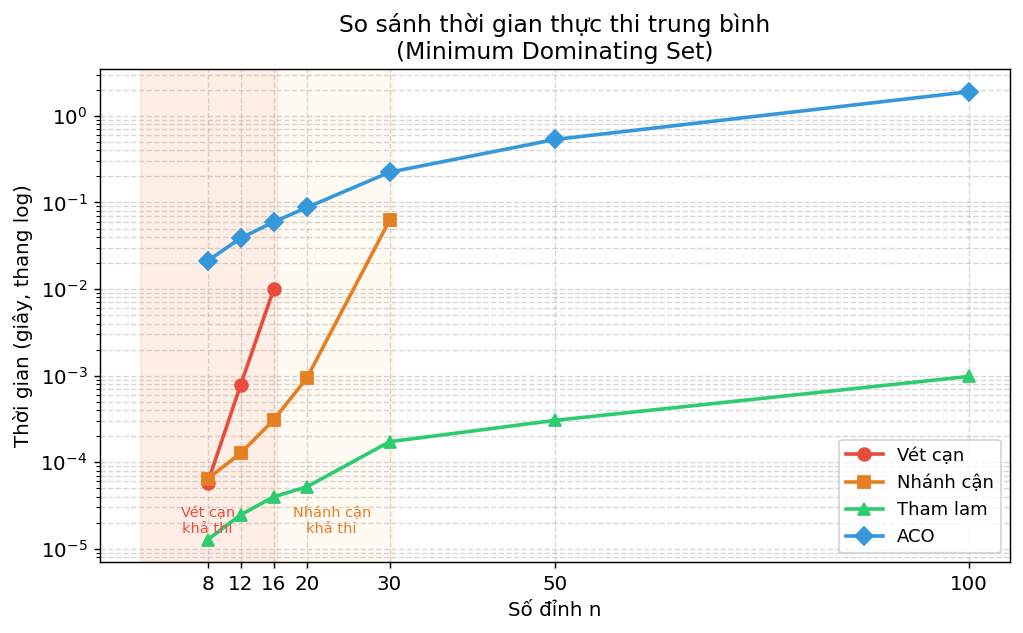
\includegraphics[width=0.9\textwidth]{results/plots/time_comparison.png}
  \caption{So sánh thời gian thực thi trung bình của các thuật toán}
  \label{fig:time}
\end{figure}

Biểu đồ thời gian dùng thang log cho thấy sự khác biệt rõ rệt giữa nhóm thuật toán chính xác và nhóm
heuristic. Vét cạn tăng nhanh do phải xét số lượng tập con rất lớn. Nhánh cận giảm mạnh số trạng thái
trong nhiều đồ thị nhờ pruning, nhưng vẫn không phù hợp khi $n$ quá lớn. Tham lam gần như tuyến tính
theo cảm nhận thực nghiệm trên bộ test này. ACO có chi phí ổn định hơn thuật toán chính xác nhưng lớn hơn
tham lam do phụ thuộc số kiến và số vòng lặp.

\section{Biểu đồ chất lượng nghiệm}

\begin{figure}[H]
  \centering
  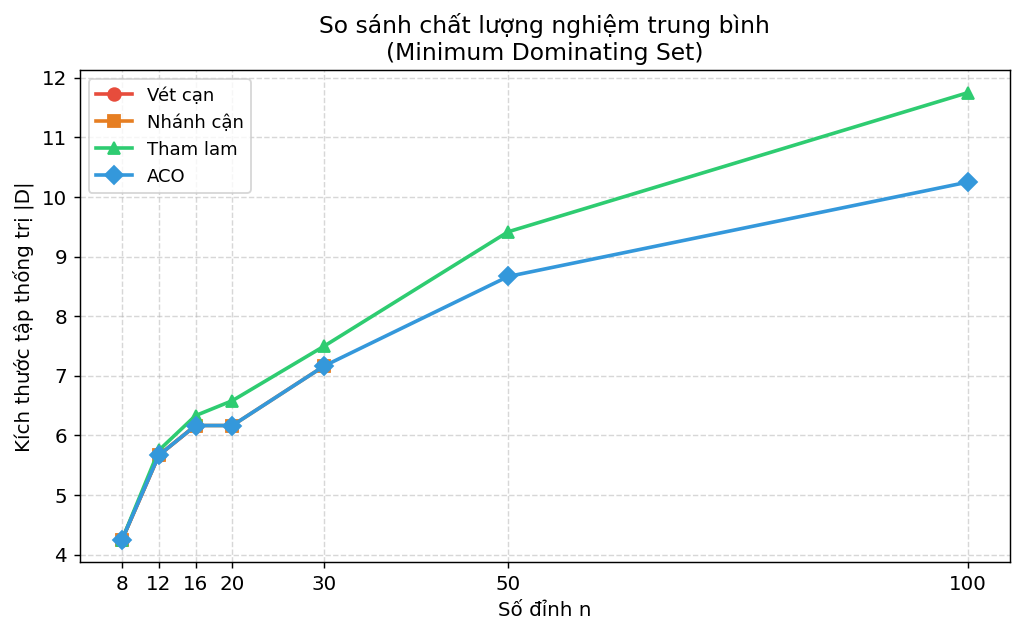
\includegraphics[width=0.9\textwidth]{results/plots/size_comparison.png}
  \caption{So sánh kích thước tập thống trị tìm được}
  \label{fig:size}
\end{figure}

Kích thước nghiệm giảm khi mật độ cạnh tăng. Điều này phù hợp với lý thuyết: đồ thị càng dày thì một
đỉnh càng có thể phủ nhiều đỉnh hơn, do đó cần ít đỉnh thống trị hơn. Ở các đồ thị thưa, số đỉnh cần chọn
lớn hơn vì mỗi đỉnh có bậc thấp và vùng phủ nhỏ.

\section{Phân tích theo mật độ cạnh}

\subsection{Đồ thị thưa}

Với $p=0.05$, đồ thị có ít cạnh, nhiều đỉnh cô lập hoặc gần cô lập. Khi đó mọi thuật toán thường phải chọn
nhiều đỉnh hơn. Ở $n=100$, tham lam cho kích thước trung bình khoảng $22.33$, trong khi ACO cho khoảng
$19.67$. Điều này cho thấy ACO có thể cải thiện chất lượng nghiệm trên đồ thị lớn và thưa, đổi lại thời
gian chạy cao hơn nhiều.

\subsection{Đồ thị mật độ trung bình}

Với $p=0.10$ và $p=0.30$, khác biệt giữa tham lam và ACO rõ hơn ở một số kích thước. Ví dụ với $p=0.10$,
$n=100$, tham lam đạt kích thước trung bình khoảng $14.33$, còn ACO đạt khoảng $12.00$. Với $p=0.30$,
$n=100$, tham lam khoảng $6.33$, ACO khoảng $5.67$.

\subsection{Đồ thị dày}

Với $p=0.50$, số thống trị rất nhỏ. Các thuật toán thường tìm được nghiệm gần nhau vì một đỉnh có thể phủ
nhiều đỉnh. Ở $n=100$, tham lam đạt khoảng $4.00$, ACO đạt khoảng $3.67$. Lợi ích chất lượng của ACO vẫn
có nhưng không quá lớn so với chi phí thời gian.

\section{So sánh chi tiết}

\begin{table}[H]
  \centering
  \caption{Đánh giá định tính sau thực nghiệm}
  \begin{tabular}{p{3cm} p{3cm} p{3cm} p{4cm}}
    \toprule
    \textbf{Thuật toán} & \textbf{Tốc độ} & \textbf{Chất lượng nghiệm} & \textbf{Khuyến nghị sử dụng} \\
    \midrule
    Vét cạn & Chậm nhất & Tối ưu & Dùng cho $n \leq 16$ hoặc kiểm chứng kết quả. \\
    Nhánh cận & Chậm đến trung bình & Tối ưu & Dùng cho đồ thị nhỏ/trung bình khi cần nghiệm chính xác. \\
    Tham lam & Nhanh nhất & Xấp xỉ khá & Dùng cho đồ thị lớn khi ưu tiên tốc độ. \\
    ACO & Trung bình đến chậm & Xấp xỉ tốt hơn trong một số trường hợp & Dùng khi chấp nhận chạy lâu hơn để tìm nghiệm nhỏ hơn tham lam. \\
    \bottomrule
  \end{tabular}
\end{table}

\section{Nhận xét về gap}

Trên các đồ thị mà thuật toán chính xác chạy được, \texttt{gap} của vét cạn và nhánh cận luôn bằng 0 do
đây là hai thuật toán tối ưu. Tham lam có gap bằng 0 ở nhiều trường hợp nhỏ hoặc đồ thị dễ, nhưng có thể
lệch so với tối ưu, ví dụ $p=0.10,n=30$ có gap trung bình khoảng $+1.33$. ACO trong bộ kết quả hiện tại
thường đạt gap 0 trên các trường hợp có đối chiếu tối ưu, nhờ kết hợp xác suất, nhiều lần thử và local
search. Tuy nhiên điều này không phải chứng minh tối ưu tổng quát cho ACO.

% =============================================================
\chapter{Kết luận}

\section{Kết quả đạt được}

Đề tài đã hoàn thành các nội dung chính:

\begin{enumerate}[leftmargin=*, label=\arabic*.]
  \item Phân tích và mô hình hóa bài toán \MDS{} trên đồ thị vô hướng, không trọng số.
  \item Thiết kế và cài đặt bốn thuật toán: vét cạn, nhánh cận, tham lam và ACO.
  \item Chứng minh tính đúng đắn cho vét cạn và nhánh cận; phân tích tính hợp lệ của tham lam và ACO.
  \item Phân tích độ phức tạp, ưu điểm và nhược điểm của từng thuật toán.
  \item Xây dựng benchmark tự động, sinh dữ liệu thực nghiệm, lưu kết quả CSV, bảng tổng hợp và biểu đồ.
\end{enumerate}

\section{Kết luận lựa chọn thuật toán}

Không có một thuật toán duy nhất tốt nhất cho mọi trường hợp:

\begin{itemize}
  \item Nếu cần nghiệm tối ưu và đồ thị rất nhỏ, vét cạn là lựa chọn đơn giản và đáng tin cậy.
  \item Nếu cần nghiệm tối ưu với đồ thị nhỏ đến trung bình, nhánh cận tốt hơn vét cạn nhờ cắt nhánh.
  \item Nếu đồ thị lớn và cần kết quả nhanh, tham lam là lựa chọn thực tế nhất.
  \item Nếu muốn cải thiện chất lượng nghiệm trên đồ thị lớn và chấp nhận thời gian chạy cao hơn, ACO là
    hướng heuristic phù hợp.
\end{itemize}

\section{Hướng phát triển}

Một số hướng mở rộng có thể thực hiện:

\begin{itemize}
  \item Cải thiện cận dưới cho nhánh cận bằng matching, packing hoặc kỹ thuật reduction.
  \item Tối ưu cài đặt tham lam bằng hàng đợi ưu tiên để giảm chi phí tính lại gain.
  \item Bổ sung các heuristic khác như simulated annealing, genetic algorithm hoặc local search nhiều
    bước.
  \item Thực nghiệm thêm trên đồ thị thực tế như mạng xã hội, mạng giao thông hoặc mạng hạ tầng.
  \item Mở rộng sang các biến thể: weighted dominating set, connected dominating set và directed
    dominating set.
\end{itemize}

% ===== REFERENCES =====
\begin{thebibliography}{99}

\bibitem{garey1979computers}
Garey, M. R., \& Johnson, D. S. (1979).
\textit{Computers and Intractability: A Guide to the Theory of NP-Completeness}.
W. H. Freeman.

\bibitem{cormen2022introduction}
Cormen, T. H., Leiserson, C. E., Rivest, R. L., \& Stein, C. (2022).
\textit{Introduction to Algorithms}.
MIT Press.

\bibitem{haynes1998fundamentals}
Haynes, T. W., Hedetniemi, S. T., \& Slater, P. J. (1998).
\textit{Fundamentals of Domination in Graphs}.
Marcel Dekker.

\bibitem{vazirani2001approximation}
Vazirani, V. V. (2001).
\textit{Approximation Algorithms}.
Springer.

\bibitem{dorigo2004ant}
Dorigo, M., \& Stutzle, T. (2004).
\textit{Ant Colony Optimization}.
MIT Press.

\end{thebibliography}

\end{document}
